% ===========================================
% Literature Review Quad Chart
% Written by: Braidan Duffy
%
% Date: 01/05/2023
% Last Revision: 01/05/2023
% ============================================

\documentclass[
	letterpaper, % Page size
	fontsize=10pt, % Base font size
	twoside=true, % Use different layouts for even and odd pages (in particular, if twoside=true, the margin column will be always on the outside)
	%open=any, % If twoside=true, uncomment this to force new chapters to start on any page, not only on right (odd) pages
	%chapterentrydots=true, % Uncomment to output dots from the chapter name to the page number in the table of contents
	numbers=noenddot, % Comment to output dots after chapter numbers; the most common values for this option are: enddot, noenddot and auto (see the KOMAScript documentation for an in-depth explanation)
]{kaobook}

\usepackage{pdfpages}
\usepackage{array}

\begin{document}

\pagelayout{wide} % Remove margin

\chapter*{Literature Review Quad Chart}

\section*{Overview}
\textbf{\emph{GRADUATE STUDENTS ONLY!}} For this assignment, you will search the literature of technical and refereed journals to find a paper on surfing physics, surfability, surf technology, or other related topic.
Prepare a quad chart that summarizes the article and explains it main topic and contribution(s) to the field. 

You may use the example below \underline{\textbf{\emph{as a reference}}}

\emph{Hint:} Do the background research ahead of the research topic proposal and use the articles you find for this review!

\section*{Requirements}
The chart must conform to the following format:

\vspace{0.5cm}

{
\setlength\extrarowheight{4pt}
\begin{table}[h!]
	\label{tab:quad_chart format}
	\begin{tabular}{| p{0.3\linewidth} | p{0.3\linewidth} |}
		\hline
		\textbf{Introduction} \newline Paper title, author(s) name, your name, executive summary. & 
		\textbf{Explanation of Main Topic} \newline Describe the main topic of the paper in detail. Use pictures or figures from the article to assist. \\
		\hline
		\textbf{Relevancy to Class} \newline How is this paper relevant to the class and (preferably) to your research topic? &
		\textbf{Contributions to Society} \newline What was the background motivation for the paper? Did they provide anything useful? What, in your opinion, is the most valuable take-away? \\
		\hline
	\end{tabular}
\end{table}
}

\section*{Grading}
This assignment will use a pass-fail scheme.
Your quad chart must adequately summarize the article and give enough detail that the instructor can understand the gist.
If you fail to do so, or do not submit a quad chart, your grade will be a 0 with the option of a redo for half-credit.

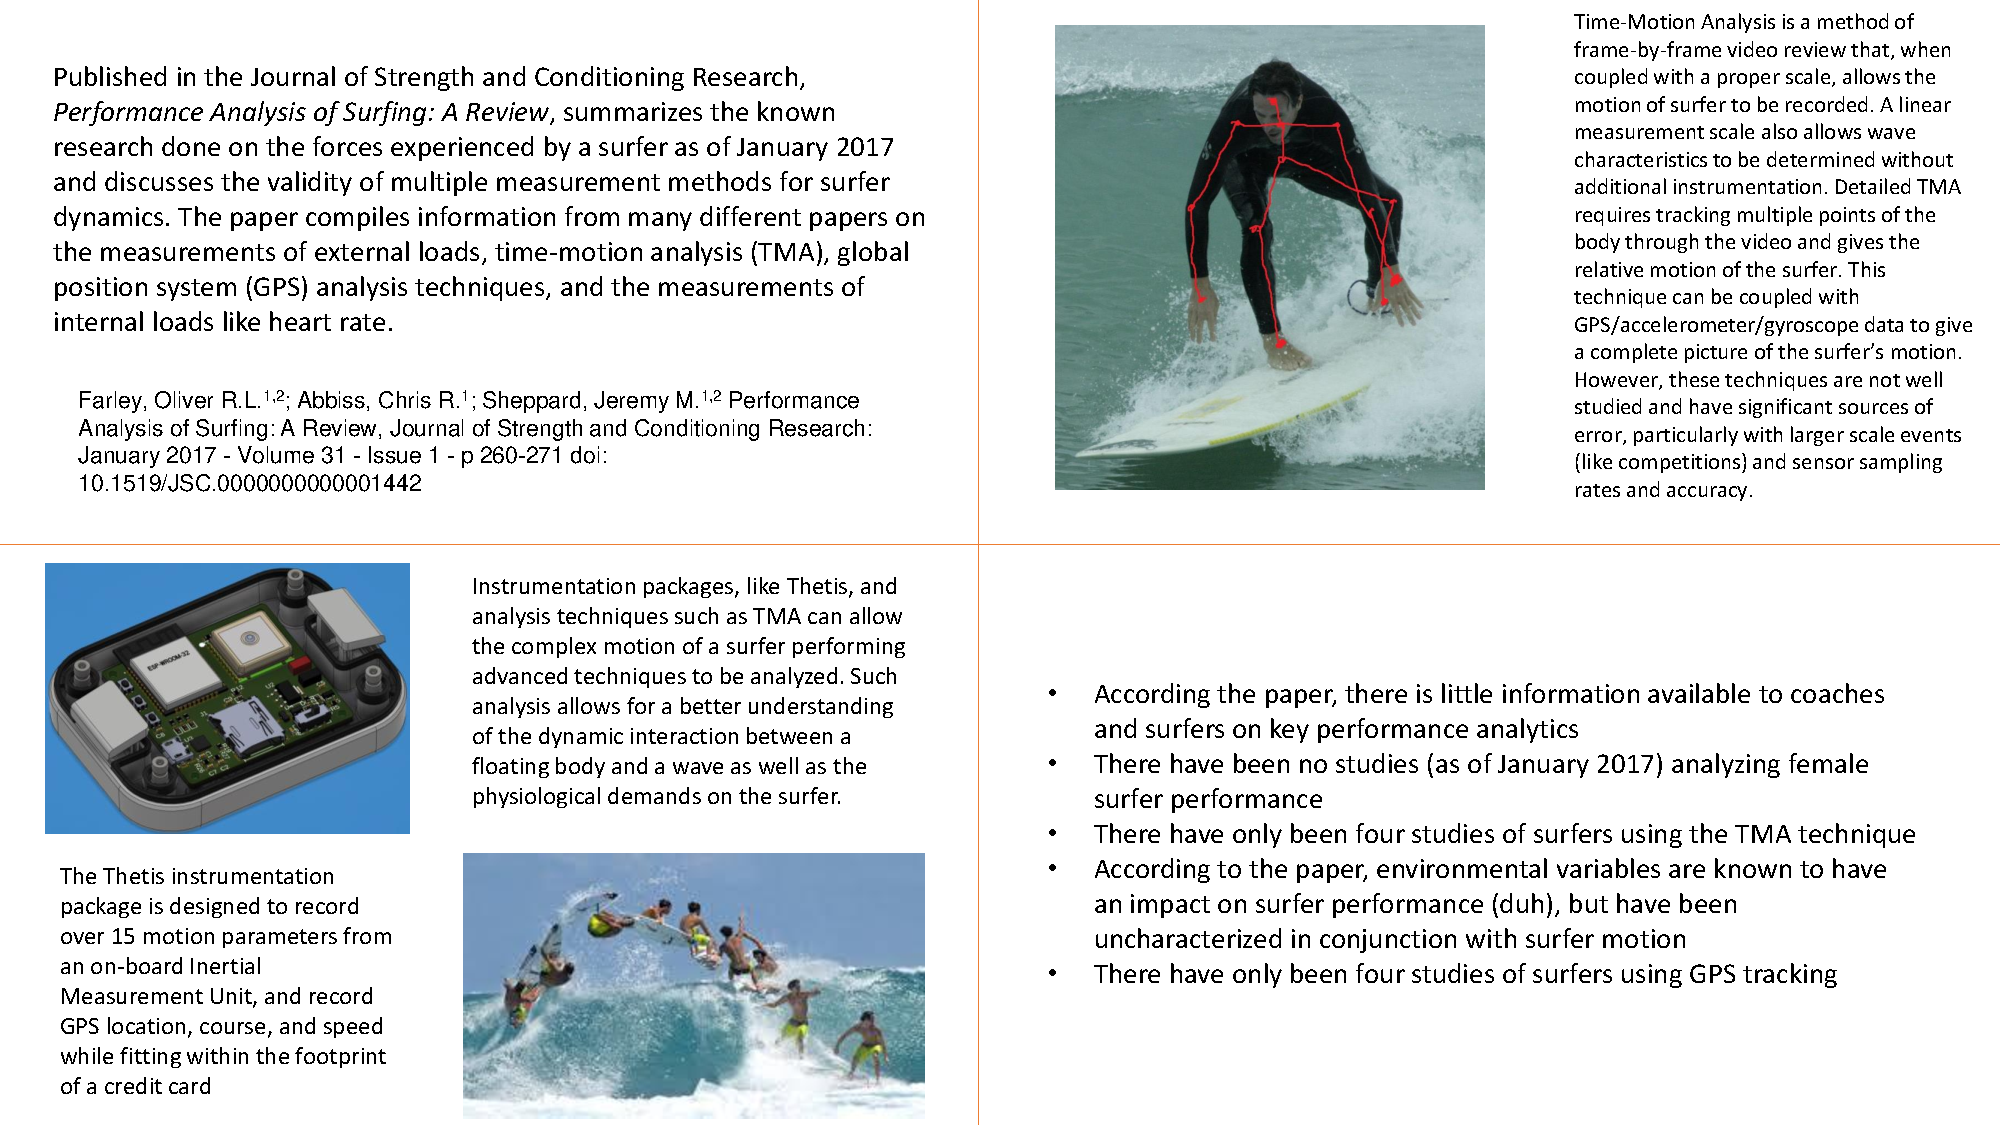
\includepdf[landscape=true]{../../publish/lit_review_qc_example.pdf}

\end{document}